\def\year{2020}\relax

\documentclass[letterpaper]{article}

\usepackage{aaai20}
\usepackage{times}
\usepackage{helvet}
\usepackage{courier}
\usepackage[hyphens]{url}
\usepackage{graphicx}
\urlstyle{rm}
\def\UrlFont{\rm}

\usepackage{graphicx}
\frenchspacing
\setlength{\pdfpagewidth}{8.5in}
\setlength{\pdfpageheight}{11in}

\usepackage{amsmath,amssymb,amsthm}
\usepackage[vlined,algoruled,titlenumbered,noend,portugues]{algorithm2e}
\usepackage{booktabs}

\graphicspath{{./images/}}

\pdfinfo{
  /Title (Relatório 02 - Algoritmos de Aprendizado por Reforço)
  /Author (Daniel Baptista Dias)
}

% /Title (Relatório 01 - Algoritmos de Planejamento Probabilístico)
% /Author (Daniel Baptista Dias)

\setcounter{secnumdepth}{0} %May be changed to 1 or 2 if section numbers are desired.

% The file aaai20.sty is the style file for AAAI Press proceedings, working notes, and technical reports.
\setlength\titlebox{2.5in} % If your paper contains an overfull \vbox too high warning at the beginning of the document, use this
% command to correct it. You may not alter the value below 2.5 in

\title{Relatório 02 - Algoritmos de Aprendizado por Reforço}
\author{Daniel Baptista Dias}

\begin{document}

\maketitle

\section{Introdução}
\label{sec:introducao}

Na disciplina de Inteligência Artificial existem algumas áreas que estudam formas de como um agente pode tomar um conjunto 
de decisões em sequência interagindo com um ambiente com o objetivo de solucionar um problema da melhor forma possível.

Uma forma de modelar esta situação é utilizando os Processos Markovianos de Decisão (MDP, do inglês \textit{Markov Decision Processes})\cite{Puterman-1994}, onde é assumido o resultado da interação do agente com o ambiente é incerto, e que uma ação realizada pelo agente neste ambiente em uma situação (um estado do ambiente) pode ter diferentes resultados, cuja frequência é ditada por uma distribuição de probabilidades, e retorna uma recompensa para o agente.

No trabalho anterior o objeto de estudo foi a área de Planjemamento Probabilístico que busca dado o conhecimento de um MDP, busca encontrar qual é a melhor forma de agir dado cada situação possível neste ambiente. Porém em algumas situações encontrar essa melhor solução pode ser complexo, seja por o número de situações possíveis ser muito alto, seja por não termos muitos dados do ambiente para poder montar uma estratégia nele.

A área de Aprendizado por Reforço busca atacar esses problemas assumindo que o agente poderá interagir nesse ambiente mesmo sem um conhecimento (ilustrada pela figura \ref{fig:rf-agent-interaction}), de forma que ele possa executar ações nele e a medida que vá interagindo com o ambiente, vá aprendendo mais características (estados, transições e recompensas) sobre ele e vá buscando encontrar melhores maneiras de agir.

\begin{figure}[t]
  \centering
  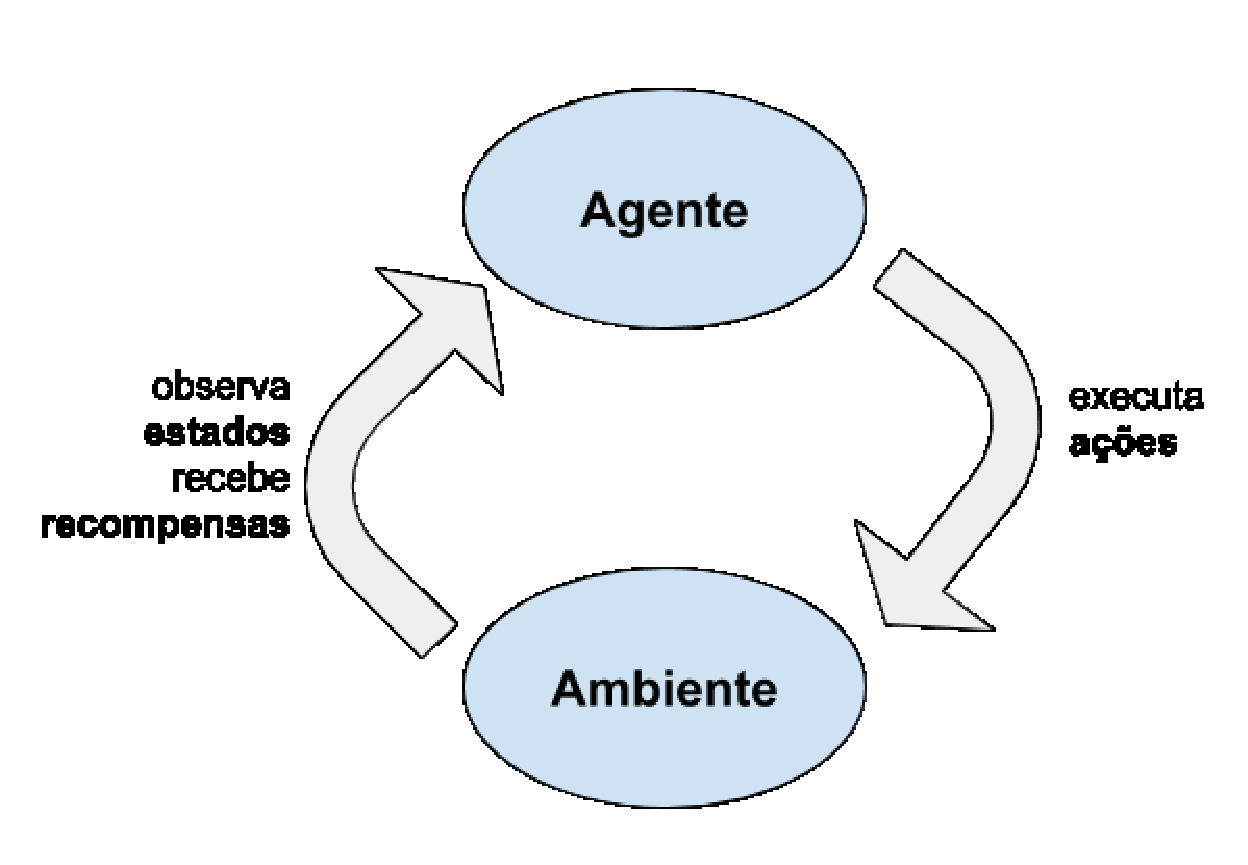
\includegraphics[width=0.9\columnwidth]{rf-agent-interaction}
  \caption{Interação de um agente com o seu ambiente}
  \label{fig:rf-agent-interaction}
\end{figure}

Neste trabalho, para efeito de estudo, serão feitos alguns experimentos com os algoritmos baseados em valor, em busca de política e com reuso de experiências.

\section{Arcabouço Teórico}

No contexto de tomada de decisões por um agente em um ambiente completamente observável, um Processo de Decisão Markoviano (MDP) pode ser descrito por uma tupla $\mathcal{M}=\langle S,A,R,P,\gamma \rangle$, onde:

\begin{itemize}
    \item $S$ é um conjunto de estados finitos e discretos, que definem a situação do ambiente em um determinado momento;
    \item $A$ é um conjunto de ações que o agente pode executar;
    \item $R : S \rightarrow \mathcal{R} $ é a função recompensa, que retorna a recompensa obtida pelo agente ao se alcançar um determinado estado;
    \item $P : S \times A \times S \rightarrow [0, 1]$ é uma função de transição que retorna a probabilidade de um agente, dado que executou uma ação $a \in A$ em um estado $s \in S$, alcançar o estado $s' \in S$. Neste trabalho uma notação que também será usada para representar essa transição é $P(s'|s,a)$.
\end{itemize}

Neste ambiente a tomada de decisão ocorre por etapas (estágios), onde o agente executa uma ação de cada vez alterando o estado do ambiente e recebendo uma recompensa ou sendo penalizado com um custo (recompensa negativa). Estes estágios são denominados pela notação $t \in \{ 1, \dots, T \} $, onde caso $T$ seja um número finito, consideramos o problema como um problema de \textbf{horizonte finito}.

O objetivo do agente neste MDP é encontrar uma política $\pi : S \rightarrow A$ que indique a melhor ação a ser tomada em cada estado $s$ a fim de se obter a maior recompensa possível.

Para identificar esta política pode-se calcular o valor dela para cada estado $s$ através do critério da recompensa esperada total. Esse critério indica o quanto de recompensa um agente pode receber em média a executar uma política $\pi$ a partir do estado $s_0 = s$ até o instante $T$ dado um fator de desconto $\gamma$ (limitado ao intervalo $[0, 1]$), calculada pela função valor $V : S \rightarrow \mathcal{R} $ para a política $\pi$:

\begin{equation} \label{eq:total_expected_reward}
    V_\pi(s) = E_{\pi} \left[ \sum_{t=0}^{T} \gamma^t r_t | s_0 = s \right]
\end{equation}

Uma política ótima $\pi^*$ para um MDP é aquela que tem o maior valor entre todas as outras políticas possíveis para cada estado, ou seja: $V_{\pi^*}(s) \geq V_{pi'}(s), \forall s,\pi'$.

O valor da política ótima $V_{\pi^*}$ pode ser encontrado a partir função valor ótima $V^* = V_{\pi^*}$ definida pela equação de Bellman \cite{Bellman-1966}, que encontra uma função valor que maximize as recompensas esperadas para todo $s \in S$:

\begin{equation} \label{eq:bellman_equation}
    V^*(s) = R(s) + \max_{a \in A} \left\{ \gamma \sum_{s'\in S} P(s'|s,a)V^*(s') \right\}
\end{equation}

Existem algoritmos que trabalham com essa abordagem para se obter a política ótima, usualmente resolvendo a equação de Bellman através de algoritmos de \textit{programação dinâmica} como o \textit{Iteração de Valor} e a \textit{Iteração de Política} \cite{Howard-1960} de forma eficiente. Neles, aplicamos um operador de Bellman para cada estado, descrito pela equação \ref{eq:bellman_operator} abaixo: 

\begin{equation} \label{eq:bellman_operator}
  V^{t+1}(s) = (BV^t)(s) = \max_{a \in A} \left\{ Q^{t+1}(s,a) \right\}
\end{equation}

onde $ Q^{t+1}(s,a) $ é considerado uma função qualidade, definida por:

\begin{equation} \label{eq:quality_function}
  Q^{t+1}(s,a) = R(s) + \gamma \sum_{s'\in S} P(s'|s,a)V^t(s')
\end{equation}

Entretanto para alguns tipo de problema eles ter uma aplicabilidade limitada devido ao problema da \textit{maldição da dimensionalidade}: o fato que o número de estados pode ser proibitivamente grande dependendo da modelagem dos estados (por exemplo, caso um estado precise modelar muitas variáveis com diferentes combinações de valores) \cite{SuttonBarto-2018}. 

Uma forma de tentar evitar o problema do crescimento do espaço de estados é ao invés de usar um conhecimento completo do ambiente para resolver-lo, buscar uma política ótima através do uso da experiência: a simulação ou interação de um agente agindo no ambiente em sequência, amostrando uma sequência de estados, ações e recompensas. Os métodos de \textit{Monte Carlo} buscam justamente fazer isso, baseando a tomada de decisão em cima das amostragens média dessa experiência ao invés de utilizar a equação de Bellman, obtendo uma estimativa da função valor $\hat{V}(s)$ e da função qualidade $\hat{Q}(s,a)$, concentrando o uso os recursos computacionais nos estados e ações mais relevantes para a resolução do problema.

%TODO: falar sobre o dilema exploração / exploitação

Esse tipo de algoritmos garante uma solução $\epsilon$-ótima independente do tamanho do espaço de estados ($|S|$) mostrando que a probabilidade de falha de convergência pode ser limitada segundo a desigualdade de Hoeffding \cite{Hoeffding-1994}. Nesses algoritmos é mostrando que caso haja uma quantidade suficientemente grande de episódios (amostras de um agente executando uma política $\pi_{\hat{Q}}$ em um ambiente) essa probabilidade de falha de convergência tende a zero. Um algoritmo que baseia nessa idéia de convergência é o UCT \cite{KocsisSzepesv-2006}.

Combinando as idéias dos métodos de Monte Carlo e de programação dinâmica (baseados no cálculo do operador de Bellman) o método de \textit{diferença temporal} buscam calcular a função valor $V$ com base na experiência de um agente em um ambiente, que através da aproximação estocástica \cite{RobbinsMonro-1951}, estima a função valor para um instante $t$, estado $s_t$, recompensa recebida $r_t$ e  uma taxa de aproximação a $V(s_t)$ (também chamada de taxa de aprendizado) $\alpha \in (0, 1])$ como:

\begin{equation} \label{eq:temporal_difference}
  V(s_t) = V(s_t) + \alpha [ r_t + \gamma V(s_{t+1}) - V(s_t) ]
\end{equation}

Dado uma política $\pi$ qualquer e um horizonte $T$, pode-se aplicar este método para avaliar esta política e encontrar $V_{\pi}$, em um algoritmo com garantia de convergência chamado \textsc{TD(0)}. Ele será a base para dois algoritmos que serão apresentados posteriormente, o \textit{SARSA} e o \textit{Q-Learning} \cite{Watkins-Dayan-1992}.

Mesmo não precisando iterar por todo o espaço de estados, armazenar e calcular $V(s)$ e $Q(s,a)$ pode demandar de muitos recursos computacionais (por exemplo, ao tentar armazenar um estado contínuo sem nenhuma técnica de discretização). Uma forma de resolver este problema é ao invés de trabalhar com uma aproximação da função valor $ \hat{V}(s, \theta) \approx V_{\pi}(s)$, onde ao invés de se armazenar os valores de $s$ serão armazenados o vetor de pesos $\theta \in \mathcal{R}^d$, onde $d$ seja menor que $|S|$. Nesta abordagem, os algoritmos se focarão em aprender os valores de $\theta$ de forma a encontrarem uma política ótima para a interação com o ambiente. Os algorimos de busca no espaço de políticas, \textit{REINFORCE com baseline}, e o que trabalha com reuso de experiências, o \textit{Fitt-Q}, partem desses principios para o aprendizado.

\section{Algoritmos}

Neste trabalho foram implementados dois algoritmos \textit{value-based} que utilizam o método de diferença temporal para identificar uma política ótima em um ambiente: os algoritmos \textit{SARSA} e \textit{Q-Learning} \cite{Watkins-Dayan-1992}, um algoritmo que trabalha com busca no espaço de políticas, o \textit{REINFORCE com baseline} e um que trabalha com reuso de experiências (\textit{sample efficient}), o \textit{Fitt-Q} \cite{Riedmiller-2005}.

\subsection{SARSA}

Partindo das técnicas de diferença temporal, a prova de convergência de diferença temporal para $V(s_t)$ no algoritmo \textsc{TD(0)} também se aplica para o aprendizado de $Q(s, a)$, onde dado um estado não terminal $s$ e simulando uma ação $a$ de política $\pi$, podemos atualizar $Q(s,a)$ segundo a equação \ref{eq:time_diff_update_sarsa}:

\begin{multline} \label{eq:time_diff_update_sarsa}
  \textsc{TimeDiff}(Q, s, a, s', \gamma, \alpha) = \\ 
  Q(s,a) = Q(s,a) + \alpha [r + \gamma Q(s', a') - Q(s,a)]
\end{multline}

Nesse algoritmo durante $T$ episódios o \textsc{SARSA} (Algoritmo \ref{alg:sarsa}) irá amostrar pares de estado-ação para cada instante $t \in \{ 1, \dots, T \}$ e os atualizará com a diferença temporal. Caso seja encontrado um estado terminal, o valor de $Q(s,a)$ será atualizado para zero e o episódio será encerrado. Como esta regra considera a quintupla $ (s, a, r, s', a') $, ela dá o nome ao próprio algoritmo \textsc{SARSA} (Algoritmo \ref{alg:sarsa}). Nele o método \textsc{TimeDiff} justamente aplica a Equação \ref{eq:time_diff_update_sarsa}. 

A tomada de decisão de uma ação nesse algorito se dá seguindo uma política $\epsilon$-gulosa sobre o valor de $Q$, onde o algoritmo \textit{explora} o espaço de estados selecionando uma ação de maneira uniforme com probabilidade $\epsilon$ e explota (escolhe a ação com base no critério $a = \arg \max_{a' \in A} Q(s, a') $) as ações com probabilidade $1 - \epsilon$. Esse método de escolha é descrito no algoritmo pelo método \textsc{ChooseActionFromPolicy}.

Durante a fase de exploração, ao escolher a ação baseada na política para atualizar o valor o estado (segmento $r + \gamma Q(s', a') - Q(s,a)$ da equação \ref{eq:time_diff_update_sarsa}), consideramos o \textsc{SARSA} um algoritmo de controle \textit{on-policy}, ou seja, ele explora em cada episódio e a atualiza os valores dos estados sempre considerando a política $\epsilon$-gulosa atual.

As propriedades de convergência deste algoritmo dependem justamente dessa natureza dele onde o valor de $Q$ depende da política seguida. Ele converge com probabilidade 1 seguindo uma política $\epsilon$-gulosa garantindo que todos os pares de estado-ação sejam visitados infinitas vezes.

%%%%%%%%%%%%%%%%%%%%%%%%%%%%%%%%%%%%%%%%%%%%%%%%%%%%%%%%%
\linesnumbered
\dontprintsemicolon
\begin{algorithm}[t!]
{
	\caption{\textsc{SARSA}($ env, T, \gamma, \alpha, \epsilon $)}
	\label{alg:sarsa}
    $Q(s,a) := 0, \forall s \in S, a \in A $\\

    \ParaCada{$ t \in \{ 1, \dots, T \} $}
    {
      $s := env.start()$\\
      $a := \textsc{ChooseActionFromPolicy}(Q, \epsilon, s) $\\

      \Enqto{$ \neg env.done() $}
      {
        $s', r := env.step(a)$\\
        $a' := \textsc{ChooseActionFromPolicy}(Q, \epsilon, s') $\\
        $Q(s, a) = \textsc{TimeDiff}(Q, s, a, s', a', \gamma, \alpha)$\\
        $s := s'$ \\
        $a := a'$ \\
      }
    }

    \Retorna{$Q$}
}
\end{algorithm}
%%%%%%%%%%%%%%%%%%%%%%%%%%%%%%%%%%%%%%%%%%%%%%%%%%%%%%%%%

\subsection{Q-Learning}

O algoritmo \textsc{Q-Learning} (Algoritmo \ref{alg:q-learning}) segue a mesma idéia de atualização da função $Q(s,a)$ através da diferença temporal, porém utilizando uma estratégia \textsc{off-policy}. Ao invés de atualizar o estado na fase de exploração considerando uma ação da política $\epsilon$-gulosa atual, ele considera o valor de $Q(s,a)$ da melhor ação naquele momento, considerando a atualização de diferença temporal como a equação \ref{eq:time_diff_update_q_learning}:

\begin{multline} \label{eq:time_diff_update_q_learning}
  \textsc{TimeDiff}(Q, s, a, s', \gamma, \alpha) = \\ 
      Q(s,a) = Q(s,a) + \alpha [r + \gamma max_a' Q(s', a') - Q(s,a)]
\end{multline}

Note que nesta versão do update, o método \textsc{TimeDiff} não necessita mais de $a'$, por considerar agora o maior valor $Q$ dentre as ações disponíveis. Essa alteração simplifica as provas de convergência e a sua análise e vai servir de base para outros algoritmos baseados em Q-Learning, como o \textsc{Fitt-Q} que será mostrado adiante.

Exceto pela atualização por diferenção temporal, o restante do algoritmo é semelhante ao \textsc{SARSA}: durante a fase de exploração a escolha da próxima ação segue a política $\epsilon$-gulosa atual e as propriedades de convergência se mantêm as mesmas, é necessário visitar todos os pares de estado-ação infinitas vezes para convergir por probabilidade 1.

%%%%%%%%%%%%%%%%%%%%%%%%%%%%%%%%%%%%%%%%%%%%%%%%%%%%%%%%%
\linesnumbered
\dontprintsemicolon
\begin{algorithm}[t!]
{
	\caption{\textsc{Q-Learning}($ env, T, \gamma, \alpha, \epsilon $)}
	\label{alg:q-learning}
    $Q(s,a) := 0, \forall s \in S, a \in A $\\

    \ParaCada{$ t \in \{ 1, \dots, T \} $}
    {
      $s := env.start()$\\

      \Enqto{$ \neg env.done() $}
      {
        $a := \textsc{ChooseActionFromPolicy}(Q, \epsilon, s) $\\
        $s', r := env.step(a)$\\
        $Q(s, a) = \textsc{TimeDiff}(Q, s, a, s', \gamma, \alpha)$\\
        $s := s'$ \\
      }
    }

    \Retorna{$Q$}
}
\end{algorithm}
%%%%%%%%%%%%%%%%%%%%%%%%%%%%%%%%%%%%%%%%%%%%%%%%%%%%%%%%%

\subsection{REINFORCE}

O algoritmo \textsc{REINFORCE} trabalha a partir das abordagens de aproximação de função, neste caso aprendendo um vetor de pesos $\theta \in \mathcal{R}^d$, com um $d < |S \times A|$ que aproxime uma função de política $P(s|a, \theta)$, ou seja realizando uma busca no espaço de políticas. Nele é considerada uma função avaliadora $J(]theta)$ de forma a se se possa aproximar com um método de gradiente ascendente en $J$:

\begin{equation}
  \theta_{t+1} = \theta_t + \alpha \widehat{\nabla J(\theta_t)}
\end{equation}

Onde $\widehat{\nabla J(\theta_t)} \in \mathcal{R}^d$ é uma estimativa estocástica cuja esperança aproxima o gradiente da medida de performance com respeito a $\theta_t$ \cite{SuttonBarto-2018}.

Pelo teorema do gradiente de política pode-se mostrar que $\nabla J(\theta_t)$ e o update de $\theta$ podem ser escritos como:

\begin{equation}
  \label{eq:reinforce_theta_j_gradient}
  \nabla J(\theta_t) = E_{\pi} \left[ G_t \frac{\nabla_{\pi}(a_t|s_t, \theta)}{\pi(a_t|s_t, \theta)} \right]
\end{equation}

\begin{equation}
  \label{eq:reinforce_theta_approximation}
  \theta_{t+1} = \theta_t + \alpha G_t \frac{\nabla_{\pi}(a_t|s_t, \theta_t)}{\pi(a_t|s_t, \theta_t)} 
\end{equation}

Onde $G_t$ é o retorno das recompensas descontados que um agente recebe ao seguir uma política $\pi(\cdot | \cdot, \theta)$ ao longo do tempo. Por fim, para a regra de atualização de $\theta_{t+1}$ pode-se substituir $\frac{\nabla_{\pi}(a_t|s_t, \theta)}{\pi(a_t|s_t, \theta)}$ por $ \nabla \ln \pi(a_t, s_t, \theta_t) $.

Com a equação de aproximação em mãos, o \textsc{REINFORCE} pode ser visto no Algoritmo \ref{alg:reinforce}, onde para cada episódio se amostra uma sequência triplas de estado, ação e recompensa para uma política $\pi(\cdot | \cdot, \theta)$ e essa sequência é utilizada para atualizar $\theta$ segundo a equação \ref{eq:reinforce_theta_approximation}.

%%%%%%%%%%%%%%%%%%%%%%%%%%%%%%%%%%%%%%%%%%%%%%%%%%%%%%%%%
\linesnumbered
\dontprintsemicolon
\begin{algorithm}[t!]
{
	\caption{\textsc{Reinforce}($ env, T, \gamma, \alpha $)}
	\label{alg:reinforce}
    inicializa $ \theta $ com valores arbitrários \\

    \ParaCada{$ episode \in \{ 1, \dots, T \} $}
    {
      $episodeSteps := \textsc{GenerateEpisode}(env, \theta)$\\

      \ParaCada{$s_t, r_t, a_t, t \in episodeSteps$}
      {
        $G := \sum_{k = t+1}^T \{ \gamma^{k-t-1} episodeSteps[k].r \}$\\
        $ \theta := \theta + \alpha \gamma^t G \nabla \ln \pi(a_t|s_t, \theta) $
      }
    }
}
\end{algorithm}
%%%%%%%%%%%%%%%%%%%%%%%%%%%%%%%%%%%%%%%%%%%%%%%%%%%%%%%%%

Além da aproximação da política utilizando um $\theta$, uma outra versão do \textsc{REINFORCE}, vista no algoritmo \ref{alg:reinforce_baseline}, pode também utilizar outra função de aproximação, um baseline $b(s_t)$, que pode acelerar o aprendizado de $\theta$ (equação \ref{eq:reinforce_theta_approximation_baseline}). No caso do algoritmo \textsc{REINFORCE-B}, este baseline é uma estimativa da função valor $b(s_t) = \hat{v}(s, w)$, onde o parâmetro $w$ também é aprendido ao longo da execução do algoritmo.

Neste trabalho o código do \textit{REINFORCE com baseline} utiliza redes neurais para implementar o aprendizado de $\theta$ e $w$.

\begin{equation}
  \label{eq:reinforce_theta_approximation_baseline}
  \theta_{t+1} = \theta_t + \alpha (G_t - b(s_t)) \frac{\nabla_{\pi}(a_t|s_t, \theta_t)}{\pi(a_t|s_t, \theta_t)} 
\end{equation}

%%%%%%%%%%%%%%%%%%%%%%%%%%%%%%%%%%%%%%%%%%%%%%%%%%%%%%%%%
\linesnumbered
\dontprintsemicolon
\begin{algorithm}[t!]
{
	\caption{\textsc{Reinforce-B}($ env, T, \gamma, \alpha_{\theta}, \alpha_{w} $)}
	\label{alg:reinforce_baseline}
    inicializa $ \theta $ e $ w $ com valores arbitrários \\

    \ParaCada{$ episode \in \{ 1, \dots, T \} $}
    {
      $episodeSteps := \textsc{GenerateEpisode}(env, \theta)$\\

      \ParaCada{$s_t, r_t, a_t, t \in episodeSteps$}
      {
        $G := \sum_{k = t+1}^T \{ \gamma^{k-t-1} episodeSteps[k].r \}$\\
        $ \delta := G - \hat{v}(s_t, w) $\\
        $ w := w + \alpha_w \delta \nabla \hat{v}(s_t, w) $\\
        $ \theta := \theta + \alpha_{\theta} \gamma^t \delta \nabla \ln \pi(a_t|s_t, \theta) $
      }
    }
}
\end{algorithm}
%%%%%%%%%%%%%%%%%%%%%%%%%%%%%%%%%%%%%%%%%%%%%%%%%%%%%%%%%

\subsection{Fitt-Q}

No algoritmo \textsc{Fitt-Q} \cite{Riedmiller-2005}, assim como nos algoritmos anteriores, a idéia é aprender os vetores de peso $\theta$ de forma que seja possível minimizar o erro quadrático médio de Bellman, conforme a equação \ref{eq:msbe}:

\begin{equation} \label{eq:msbe}
  \textsc{MSBE}(\theta, \theta') = || \hat{V}_{\theta} - \mathcal{T} \hat{V}_{\theta'} ||^2_D
\end{equation}

Para este otimização é preciso calcular a norma quadrática entre estimativas de $\hat{V}_{\theta}$ e $\hat{V}_{\theta'}$ aplicado ao operador de Bellman $\mathcal{T}$ considerando $D$ uma matriz diagonal contendo uma distribuição limite $d(s) = \lim_{t \rightarrow \infty} P(s_t = s)$, utilizando o algoritmo \ref{alg:fittq-theory}.

Ao invés de usar uma técnica de gradiente descendente que utilize uma taxa de aprendizado $\alpha$ para encontrar uma valor de $\theta$, o trabalho de \cite{Riedmiller-2005} propõe aplicar uma rede neural que reuse experiências de interação de um agente com o ambiente (episódios) para treinar esta rede e encontrar uma estimativa $\hat{Q}(s, a)$ que o agente possa utilizar para agir no ambiente. 

Neste algoritmo são considerados apenas os parâmetros $T_{train}$, o horizonte máximo de amostragem de um episódio para treinamento da rede neural, e $T_{eval}$, o horizonte máximo de amostragem de um episódio de avaliação da rede.

%%%%%%%%%%%%%%%%%%%%%%%%%%%%%%%%%%%%%%%%%%%%%%%%%%%%%%%%%
\linesnumbered
\dontprintsemicolon
\begin{algorithm}[t!]
{
	\caption{\textsc{Fitt-Q}($ env, T, \epsilon $)}
	\label{alg:fittq-theory}
    inicializa $ w_0 $ com valores arbitrários \\

    \ParaCada{$ episode \in \{ 1, \dots, T \} $}
    {
      $w_t := \arg \min_{w \in \mathcal{R}^k} \textsc{MSBE}(w, w_{t-1}) $ \\
      $res := || w_t - w_{t-1} ||$ \\

      \Se{$res < \epsilon$}
      {
        \textbf{interrompe loop}
      }
    }
}
\end{algorithm}
%%%%%%%%%%%%%%%%%%%%%%%%%%%%%%%%%%%%%%%%%%%%%%%%%%%%%%%%%

\section{Experimentos e Resultados}

Os experimentos foram executados na plataforma Google Colab com o Python, na época deste relatório com 2 CPUs de 2.2 GHz e 13GB de memória. Parte dos algoritmos foi baseado em implementações existentes e estão disponíveis no Github\footnote{Disponível em https://github.com/danielbdias/automated-planning-and-reinforcement-learning-studies}. Os algoritmos base das implementações foram:

\begin{itemize}
  \item \textit{Q-Learning} e \textit{SARSA}: https://github.com/dennybritz/reinforcement-learning/tree/master/TD
  \item \textit{REINFORCE com baseline}: https://github.com/SwamyDev/reinforcement
  \item \textit{Fitt-Q}: https://github.com/seungjaeryanlee/implementations-nfq
\end{itemize}

\subsection{Configuração dos experimentos}

O domínio utilizado foi o \textit{CartPole} \cite{SuttonBarto-2018}, que consiste em controlar um carrinho em movimento em um local delimitado que contém um espécie de mastro anexada a ele de pé que pode cair de acordo com o movimento do carrinho. Ele possui as seguintes características:

\begin{itemize}
  \item O estado observado é composto por quatro variáveis contínuas (exemplificadas na figura \ref{fig:cart-pole}): posição do carrinho, velocidade do carrinho, ângulo do mastro em relação ao carrinho e velocidade angular do mastro
  \item As ações possíveis são mover o carrinho para a esquerda ou para a direita, tentando equilibrar a alavanca de forma que ela não caia para um dos lados
  \item O agente recebe 1 de recompensa caso o mastro não tenha caído e o carrinho esteja em uma zona delimitada. Caso o mastro caia ou o carrinho saia da zona delimitada, a agente não recebe mais recompensa (recompensa 0)
\end{itemize}

\begin{figure}[t]
  \centering
  \includegraphics[width=0.9\columnwidth]{cart-pole}
  \caption{Exemplo do domínio \textit{CartPole}}
  \label{fig:cart-pole}
\end{figure}

Cada algoritmo foi executado 5 vezes para cada configuração de parâmetro, com as seguintes configurações: 3000 episódios, fator de desconto $\gamma = 0.9$ e os seguintes parâmetros específicos:

\begin{itemize}
  \item \textit{SARSA} e \textit{Q-Learning}: $\alpha \in \{ 0.1, 0.2, 0.5, 0.8 \}$ e $epsilon \in \{ 0.01, 0.05, 0.1, 0.2 \}$
  \item \textit{REINFORCE com baseline}: $\alpha_{\theta} \in \{ 5, 50 \}$ e $\alpha_{w} \in \{ 0.01, 0.1 \}$
  \item \textit{Fitt-Q}: $T_{train} \in \{ 100, 200, 300 \} $ e $T_{eval} = \{ 1000, 2000, 3000 \}$
\end{itemize}

Além destas parametrizações os algoritmos \textit{SARSA} e \textit{Q-Learning} utilizam uma técnica para a discretização de cada variável de estado onde o domínio de cada variável foi separado em sete pontos e cada variável poderia ter apenas o valor de um desses pontos, o ponto mais próximo do valor real dela. 

Para a avaliação de cada algoritmo foi medido a quantidade de passos com sucesso (tamanho do episódio) em relação aos episódios amostrados pelos algoritmos. Em todos os gráficos dos experimentos são mostradas as trajetórias médias das execuções de cada algoritmo. Como no domínio de testes o agente recebe um de recompensa para cada momento em que ele não deixa cair o mastro, a recompensa será igual a quantidade de passos tomados com sucesso e por isso não será considerada.

Dois tipos de comparações serão feitos nos experimentos:
\begin{enumerate}
  \item Comparação de performance de cada algoritmo considerando a variação de seus hiperparâmetros
  \item Comparação dos algoritmos considerando apenas apenas o resultado com os melhores hiperparâmetros
\end{enumerate}

\subsection{Resultados}

% explicar quantas variações houve por algoritmo e quanto tempo em média foi gasto

bla
% TODO:
% resultados do q-learning
% resultados do sarsa
% resultados do reinforce
% resultados do fitt-q

\begin{figure}[t]
  \centering
  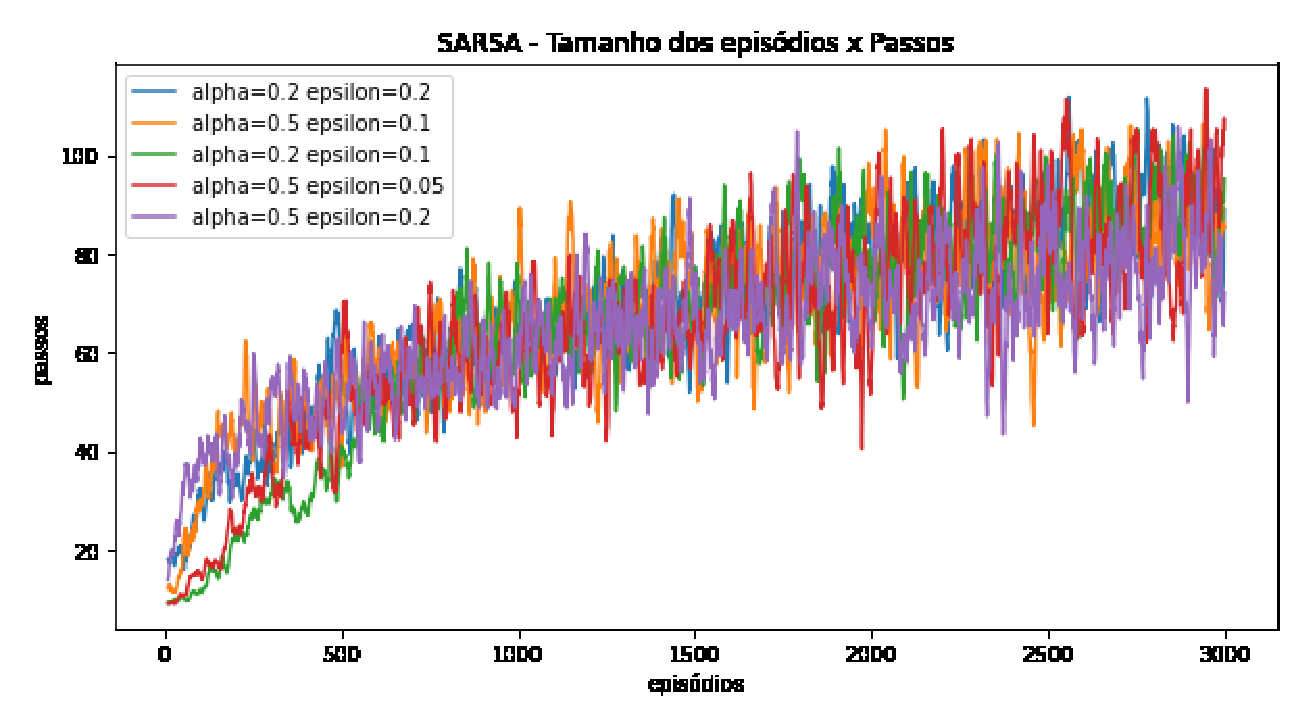
\includegraphics[width=0.9\columnwidth]{exp-sarsa-episodes}
  \caption{Tamanho de episódio - SARSA}
  \label{fig:exp-sarsa-episodes}
\end{figure}

\begin{figure}[t]
  \centering
  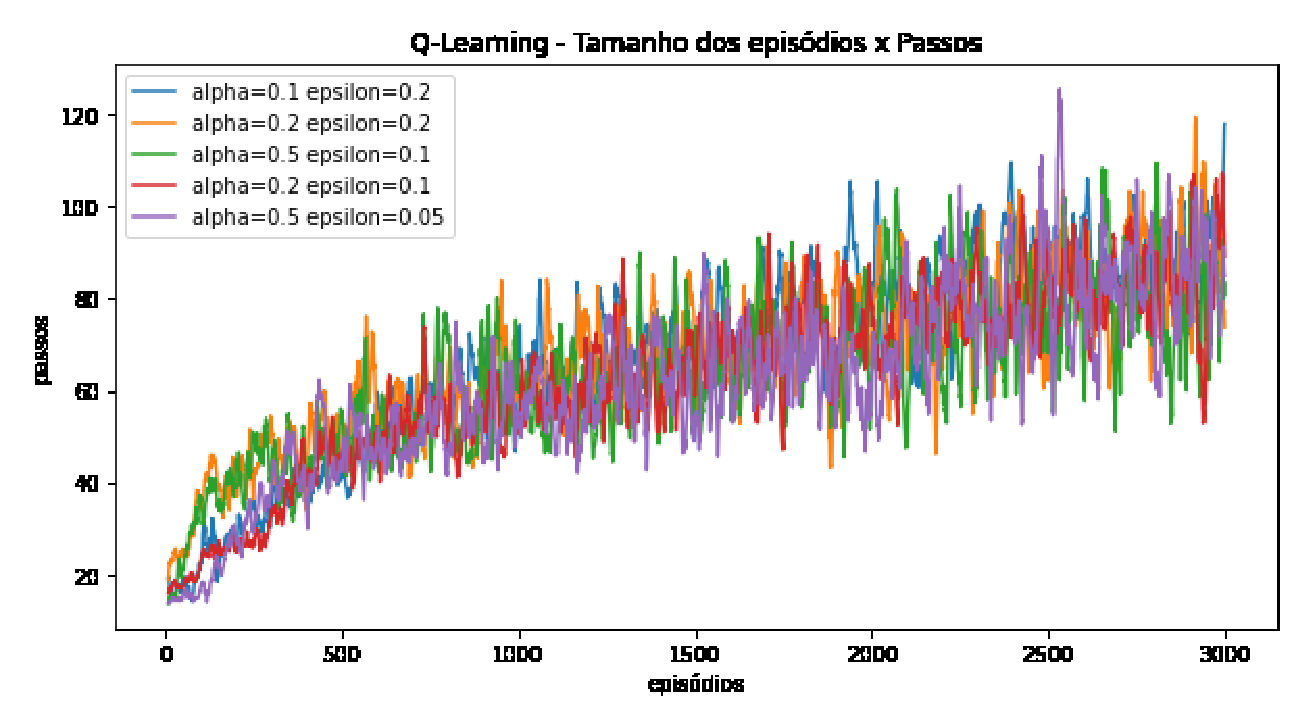
\includegraphics[width=0.9\columnwidth]{exp-qlearning-episodes}
  \caption{Tamanho de episódio - Q-Learning}
  \label{fig:exp-qlearning-episodes}
\end{figure}

\begin{figure}[t]
  \centering
  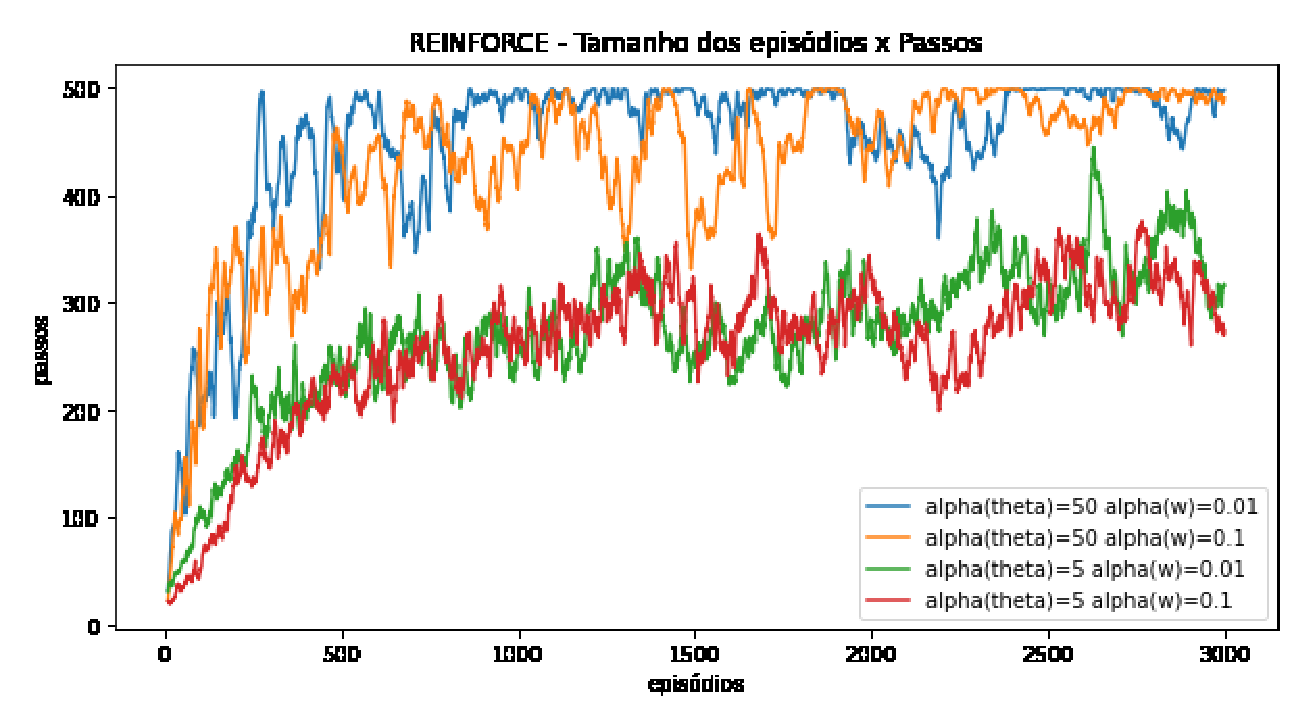
\includegraphics[width=0.9\columnwidth]{exp-reinforce-episodes}
  \caption{Tamanho de episódio - REINFORCE}
  \label{fig:exp-reinforce-episodes}
\end{figure}

\begin{figure}[t]
  \centering
  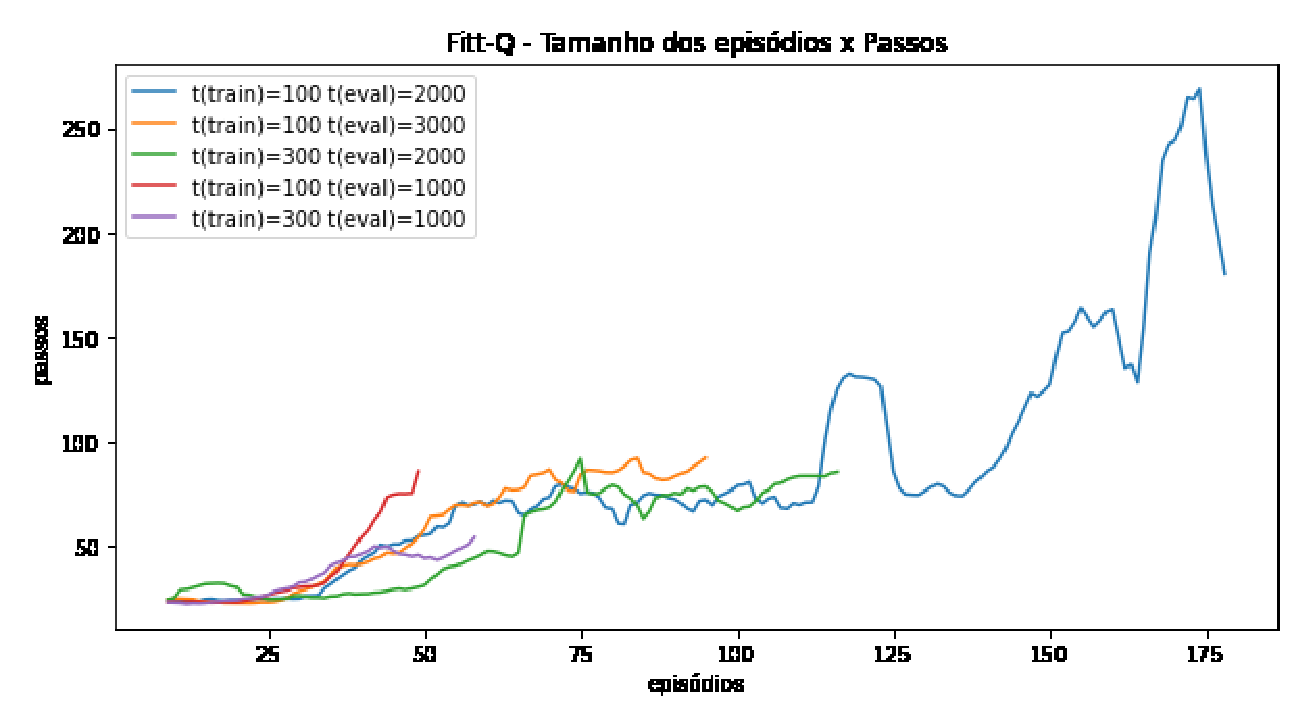
\includegraphics[width=0.9\columnwidth]{exp-fittq-episodes}
  \caption{Tamanho de episódio - Fitt-Q}
  \label{fig:exp-fittq-episodes}
\end{figure}

% montar tabela com melhores hiperparâmetros

\begin{table}[ht]
  \caption{Métricas médias dos algoritmos - Ambiente 01}
  \label{table:mean-performance-values-env01}
  \begin{tabular}{llll}
      \toprule
      Algoritmo  &                           Hiperparâmetros & Episódio \\
      \midrule
      SARSA      &          $ \alpha = 0.2, \epsilon = 0.2 $ &        ? \\
      Q-Learning &          $ \alpha = 0.1, \epsilon = 0.2 $ &        ? \\
      Reinforce  & $ \alpha_{\theta} = 50, \alpha_w = 0.01 $ &      500 \\
      Fitt-Q     & $ T_{train} = 100, T_{eval} = 2000 $      &        ? \\
      \bottomrule
  \end{tabular}
\end{table}

\begin{figure}[t]
  \centering
  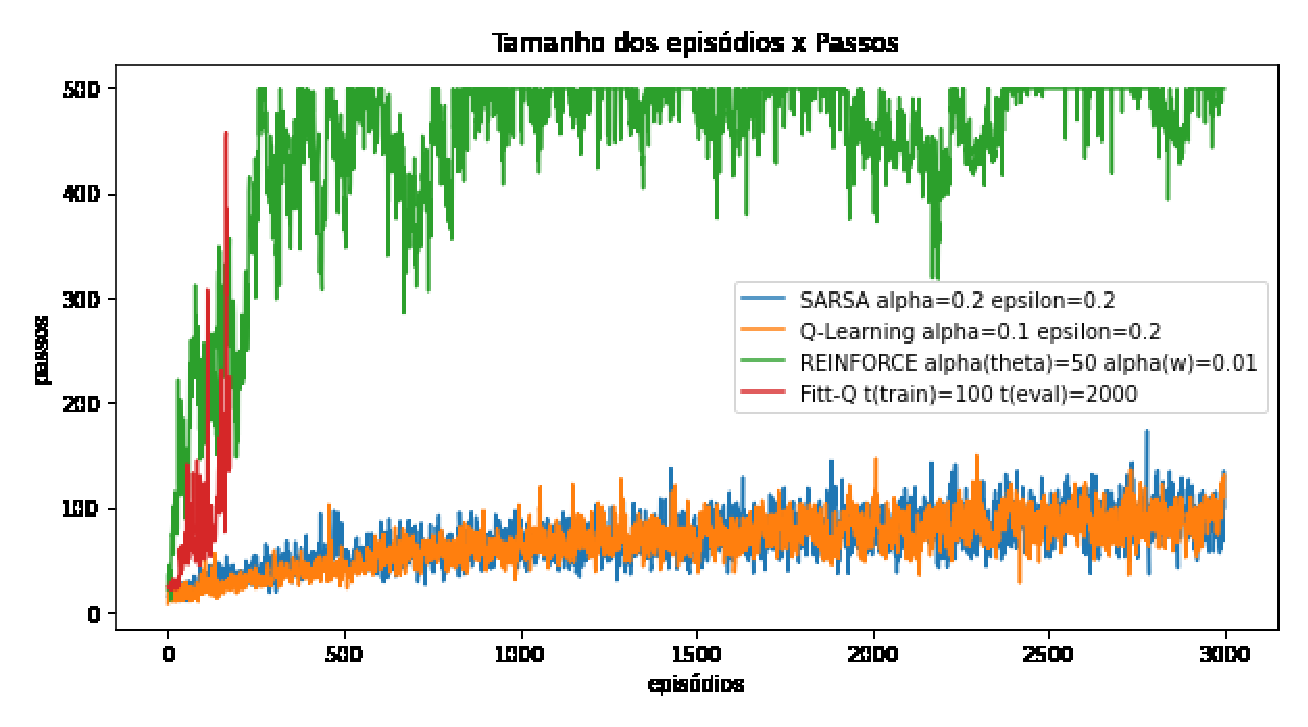
\includegraphics[width=0.9\columnwidth]{exp-allalgs-episodes}
  \caption{Tamanho de episódio - Todos algoritmos}
  \label{fig:exp-allalgs-episodes}
\end{figure}

\section{Conclusão}

bla
% TODO: avaliar experimentos e resultados

\bibliography{references.bib}
\bibliographystyle{aaai}

\end{document}
